En esta sección se detallarán los casos de uso pertenecientes al subsistema de gestión de organizaciones. La figura \ref{fig:casos_uso_subsistema_organizaciones} muestra el diagrama de casos de uso de dicho subsistema.

\begin{figure}[h]
\centering
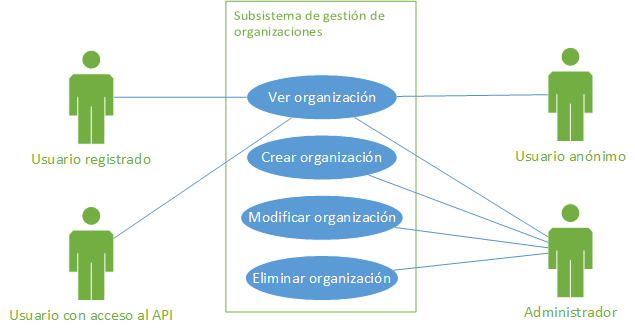
\includegraphics[width=\textwidth]{casos_uso_organizaciones}
\caption{Diagrama de casos de uso del subsistema de gestión de organizaciones}
\label{fig:casos_uso_subsistema_organizaciones}
\end{figure}


\subsubsection{Caso de uso ``ver organización''}
\begin{description}
\item[Descripción] Un usuario quiere ver la información sobre una organización.
\item[Actores] Cualquier usuario registrado o no en el sistema.
\item[Escenario principal] 	\hfill
							\begin{enumerate}
							\item El usuario pulsa en el botón que carga la vista de las organizaciones.
							\item Una vez en la vista de organizaciones pulsa en el nombre o la imagen de la organización que quiere ver en detalle.
							\item El sistema carga la vista de la organización mostrando todos sus detalles.
							\end{enumerate}
\end{description}


\subsubsection{Caso de uso ``crear organización''}
\begin{description}
\item[Descripción]  Un administrador quiere añadir una nueva organización al sistema.
\item[Actores]  El administrador del sistema.
\item[Precondiciones] Haber iniciado sesión en el sistema.
\item[Escenario principal]  \hfill
							\begin{enumerate}
							\item El usuario pulsa en el botón que carga la vista de las organizaciones.
							\item Una vez en la vista de las organizaciones pulsa el botón correspondiente para crear una organización nueva.
							\item Rellena el formulario con los datos requeridos.
							\item Si lo desea también rellena la información opcional del formulario.
							\item El administrador pulsa el botón guardar.
							\item El sistema crea la nueva noticia.
							\end{enumerate}
\item[Escenario alternativo 1] No se han rellenado todos los campos requeridos.
							\begin{enumerate}
							\item El administrador no ha rellenado todos los campos requeridos para crear una nueva organización.
							\item El sistema notificará al administrador de su error y no creará la nueva organización.
							\item Se continuará desde el punto 3 del escenario principal.
							\end{enumerate}
\end{description}


\subsubsection{Caso de uso ``modificar organización''}
\begin{description}
\item[Descripción]  Un administrador quiere modificar una organización existente en el sistema.
\item[Actores]  El administrador del sistema.
\item[Precondiciones] Haber iniciado sesión en el sistema.
\item[Escenario principal]	\hfill
							\begin{enumerate}
							\item El usuario accede a la vista de las organizaciones.
							\item Una vez en la vista de noticias localiza la organización que quiere modificar.
							\item Cuando ha accedido a la organización pulsa el botón correspondiente para modificar su contenido.
							\item Rellena toda la información requerida en el formulario.
							\item Si lo desea también rellena la información opcional del formulario.
							\item El administrador pulsa el botón guardar.
							\item El sistema actualiza la información de la organización editada.
							\end{enumerate}
\item[Escenario alternativo 1] No se han rellenado todos los campos requeridos.
							\begin{enumerate}
							\item El administrador no ha rellenado todos los campos requeridos para modificar la organización.
							\item El sistema notificará al usuario de su error y no modificará los datos de la organización.
							\item Se continuará desde el punto 4 del escenario principal.
							\end{enumerate}
\end{description}


\subsubsection{Caso de uso ``eliminar organización''}
\begin{description}
\item[Descripción]  Un administrador quiere eliminar una organización del sistema.
\item[Actores]  El administrador del sistema.
\item[Precondiciones]  Haber iniciado sesión en el sistema.
\item[Escenario principal]	\hfill
							\begin{enumerate}
							\item El administrador accede a la vista de las organizaciones.
							\item Accede a la organización que desea eliminar.
							\item Una vez en la vista de la organización pulsa el botón correspondiente para su eliminación.
							\item La organización será eliminada del sistema.
							\end{enumerate}
\end{description}